\section{Results} \label{sec:3}
The final results for the $v_{2}$ elliptic flow coefficient were obtained using the method in (\ref{subsec:2.2}) and was processed and visualized using the ROOT library. One of my tasks were to compare the results to real values in the scientific literature.

\begin{figure}[h]
	\centering
	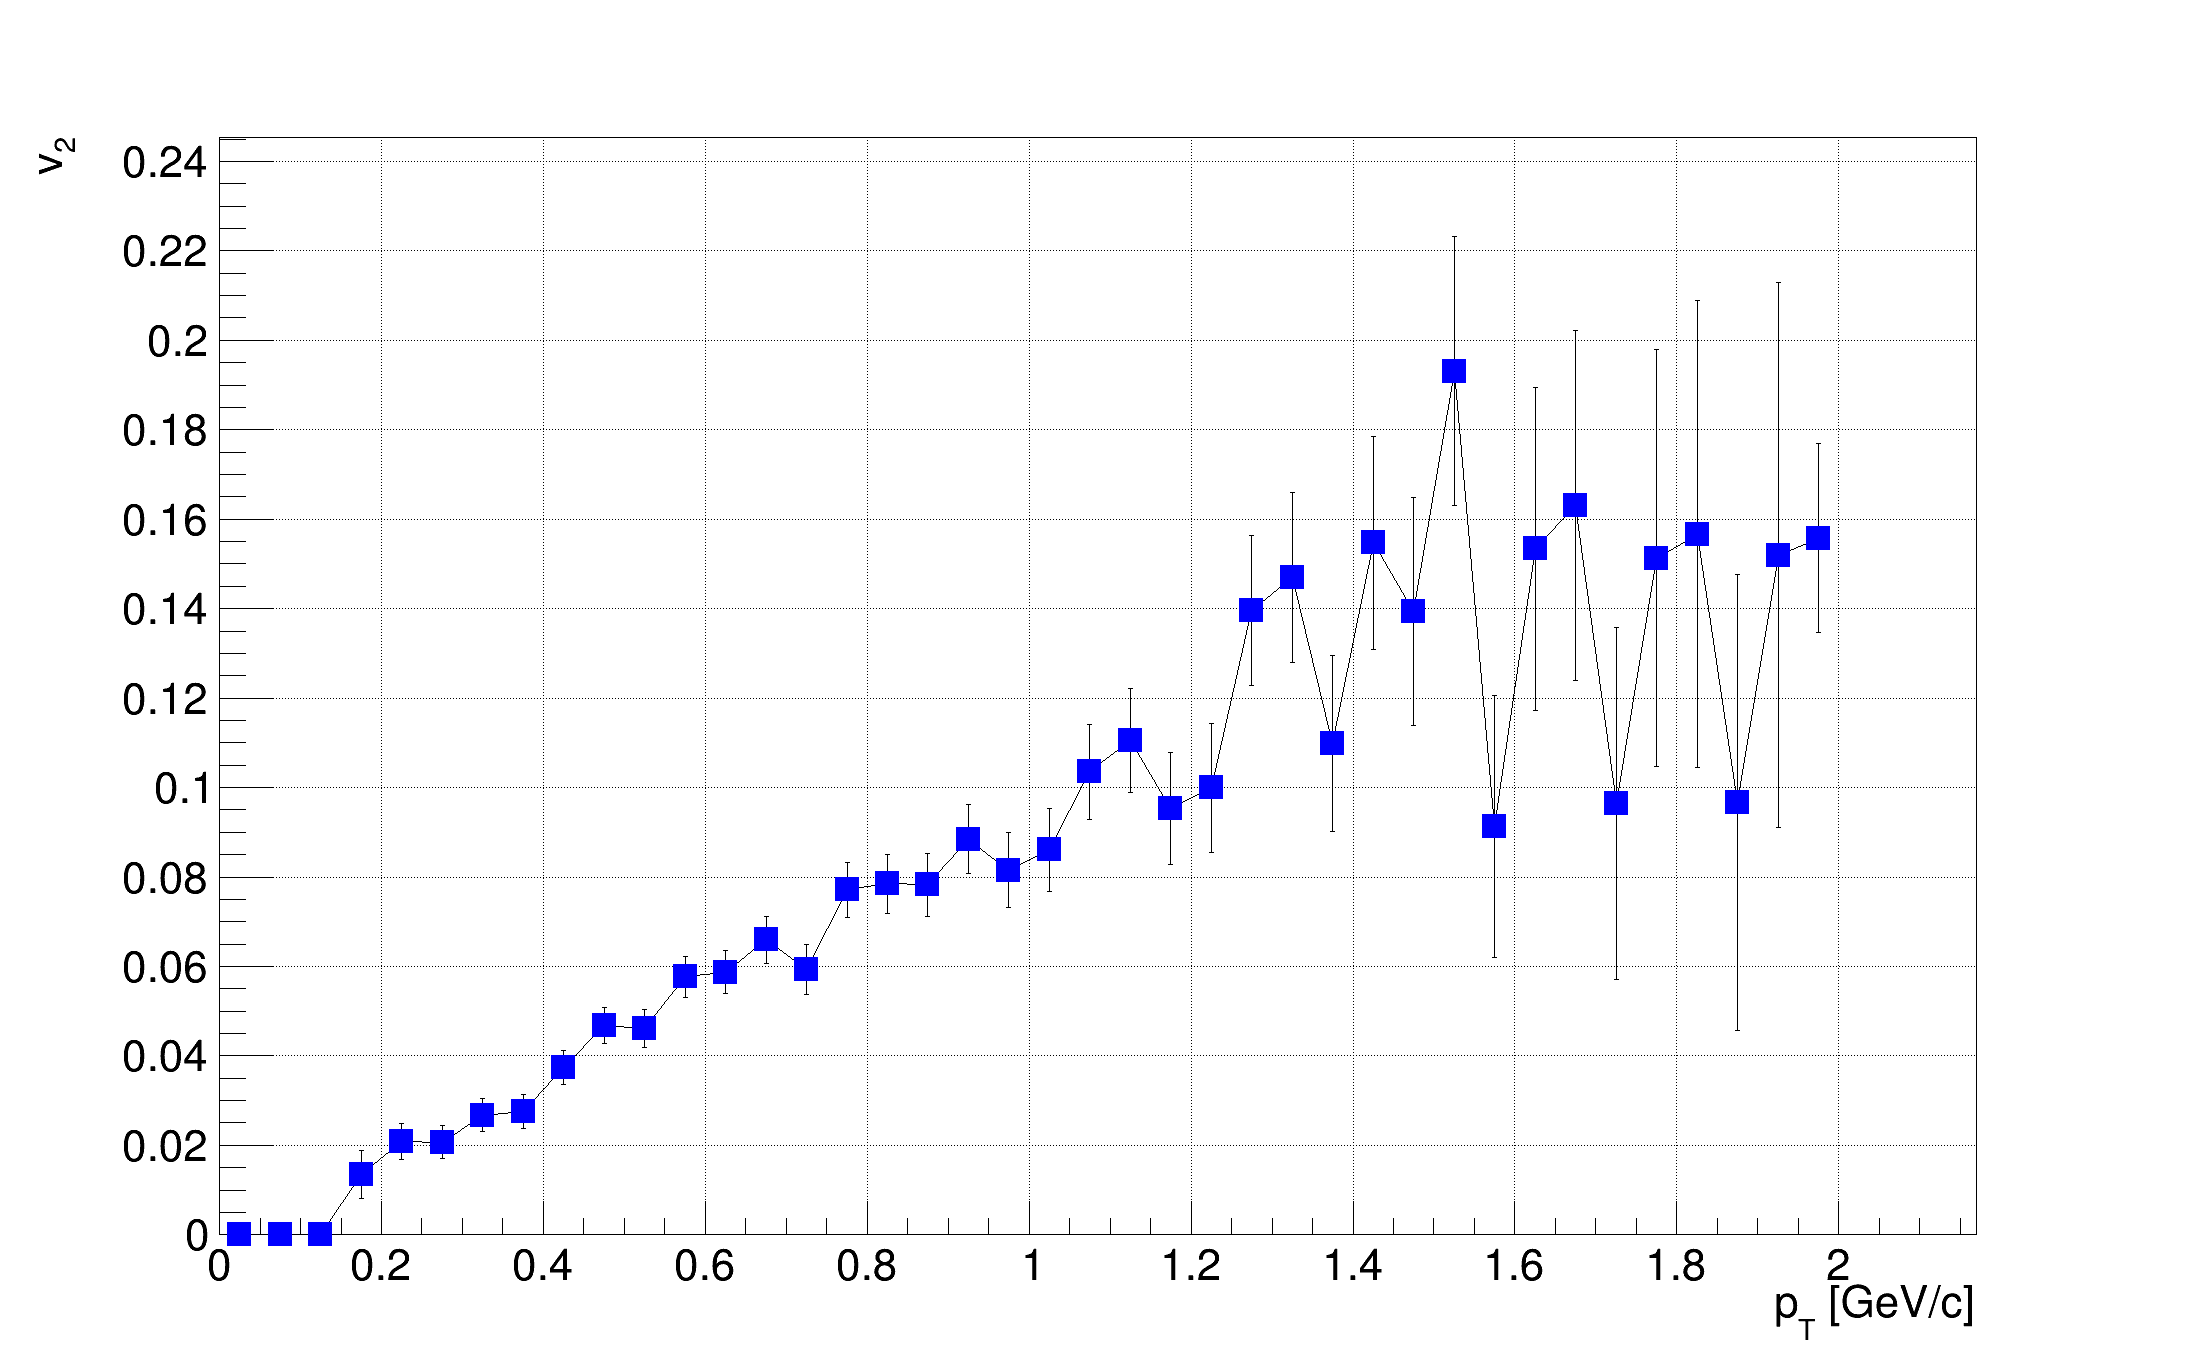
\includegraphics[width=\textwidth]{{img_src/v2_flow_per_pt.png}}
	\captionof{figure}{The $v_{2}$ elliptic flow coefficient as a function of the $p_{T}$ transverse momentum for a single centrality class of $0\% - 92\%$.}\label{fig:3}
\end{figure}
For this numerous literature can be cited, but as I've mentioned, it was advised to compare results to eg. Fig. (2) in \citep{Collaboration2003}. The very same characteristics can be observed here on Fig. (\ref{fig:3}) and in the cited article on Fig. (2). It can be seen, that the $p_{T} - v_{2}$ curve saturates as it reaches $p_{T} \approx 2\ \mathrm{GeV}/\mathrm{c}$. The maximum value of $v_{2}$ is approximately $0.16$, but the large errors in the high $p_{T}$ regime makes it impossible to estimate it more precisely.

At the end I've obtained results consistent with values in the literature, that implies my calculations were probably correct. The errors of $v_{2}$ values could be probably improved by choosing a more robust fitting method for the angle distribution, but it won't change the final implications of the project.